\documentclass{article}
\usepackage{iclr2026_conference,times}
\usepackage{hyperref}
\usepackage{url}
\usepackage{graphicx}
\usepackage{booktabs}
\usepackage{amsmath}
\usepackage{amssymb}
\usepackage{amsthm}
\usepackage{microtype}

\title{Minimum Effective Corrections for Future Robot Behavior}

\author{Anonymous Authors}

\newtheorem{proposition}{Proposition}
\newtheorem{definition}{Definition}

\begin{document}
\maketitle
\noindent\textbf{Submission-hardening v2, 2026-06-13.}
Added estimated-update-channel stress tests. The certificate is now framed as
exact only for a trusted local update map; with a noisy estimated channel, the
returned correction must be treated as a fragile local recommendation.

\begin{abstract}
Physical corrections are a natural way to teach robots, but a correction that repairs the current execution can still be invisible to the learner that determines future behavior. We formalize a \emph{Minimum Effective Correction}: the smallest physical intervention whose image through the robot's update rule crosses a specified future-behavior boundary. The resulting mechanism, Update-Boundary Correction (UBC), solves a local minimum-norm halfspace problem and returns either a correction, a nullspace warning, or an infeasibility certificate for the robot's current correction channel. In a controlled embodied-correction simulator, UBC succeeds on reachable future-behavior constraints while current-only corrections often repair the immediate margin without changing future behavior. The claims are intentionally local: the paper proves the certificate for affine update linearizations and reports simulated evidence, not a global or hardware guarantee.
A v2 stress test makes the main boundary explicit: when UBC solves with an estimated
update channel but is evaluated on the true margins, success falls to 0.330 at
channel-noise $\sigma=0.10$; a guarded variant recovers 0.750 success at larger
correction norm.
\end{abstract}

\section{Introduction}
Robots are often corrected physically: a person nudges a manipulator away from an obstacle, guides a waypoint through a safer passage, or takes over a shared-control interface. Prior work shows that such feedback can teach demonstrations, rewards, preferences, and policies \citep{argall2009survey,chernova2014robot,bajcsy2017learning,sadigh2017active,ross2011dagger,kelly2019hgdagger}. Yet these methods usually ask what the human meant, not whether the physical input lies in a part of the robot update map that can change future autonomous behavior.

This distinction matters because robot correction has two faces. One face is immediate compliance: the robot's current motion changes because a human applied force or selected an alternative command. The other is learning: future trajectories change after the contact ends. These can disagree. A small push can fix the present motion while falling in the learner's nullspace; a larger but differently directed correction can be the true minimum that changes future behavior.

This paper studies the object suggested by that disagreement. Given a robot learner, a correction interface, and a finite set of future behavior predicates, what is the smallest physical correction that changes the future policy? The answer is not generally the smallest geometric trajectory deformation. It is the smallest correction after projection through the robot's update channel.

\textbf{Contributions.} We make three contributions. First, we define the Minimum Effective Correction (MEC), a learner-relative object that distinguishes behavior-changing corrections from compliance-only motion. Second, we derive Update-Boundary Correction (UBC), a local convex certificate for affine update models and linearized future-behavior margins. Third, we provide runnable evidence showing that immediate repair can fail to produce future behavior change, while UBC either finds the minimum correction in the reachable channel or declares the request unreachable.

\section{Related Work}
\textbf{Learning from demonstration and correction.} Learning from demonstration converts human traces into policies or trajectory models \citep{argall2009survey,akgun2012keyframe,chernova2014robot}. Physical correction methods go further by treating corrective interaction as information about missing reward features or desired behavior \citep{bajcsy2017learning,bajcsy2018learning,bobu2020feature}. Our work does not claim novelty in using corrections as feedback. Instead, it asks whether a physical correction is effective under the learner's own update channel.

\textbf{Preferences and coactive improvement.} Preference-based and coactive methods use comparisons or improvements to infer reward functions \citep{jain2015learning,sadigh2017active,wirth2017survey,christiano2017deep}. They reduce the burden of full demonstrations, but the feedback object is usually a label or ranking. MEC is different: the optimization variable is the physical intervention itself, with cost measured before the learner projects it into parameter space.

\textbf{Shared autonomy and intervention-aided learning.} Shared autonomy blends human commands with autonomous inference \citep{javdani2015shared,losey2018review}. Intervention-aided imitation learning treats takeovers as corrective data \citep{ross2011dagger,kelly2019hgdagger}. These settings reveal the same risk: successful assistance or safe takeover does not prove that future autonomous behavior has changed. UBC targets that gap directly.

\textbf{Minimum intervention.} The minimum intervention principle in motor control emphasizes corrections only along task-relevant dimensions \citep{todorov2004optimality}. We borrow the spirit but change the object: the relevant dimensions are not only task-state dimensions, but the image of the robot's learning update map.

\section{Minimum Effective Correction}
Let $\theta \in \mathbb{R}^p$ denote the robot learner state, such as reward weights, planner parameters, or policy features. A physical correction $c \in \mathbb{R}^d$ is applied during an interaction $\tau$. The robot update is
\begin{equation}
    \theta^+ = U(\theta,\tau,c).
\end{equation}
For future contexts $z_j$, define behavior margins $m_j(\theta^+)$. The desired future behavior is certified when $m_j(\theta^+) \geq \gamma$ for all $j$ in a finite set $\mathcal{Z}$.

\begin{definition}[Minimum Effective Correction]
Given a correction cost matrix $W \succ 0$, the Minimum Effective Correction is
\begin{equation}
    c^\star = \arg\min_c \|c\|_W^2
    \quad \textrm{s.t.} \quad
    m_j(U(\theta,\tau,c)) \geq \gamma, \quad \forall z_j \in \mathcal{Z}.
\end{equation}
If no feasible $c$ exists inside the physical correction channel, the learner cannot certify the requested future behavior from this interface at this state.
\end{definition}

The definition is intentionally learner-relative. It does not say that the task is impossible, that the human is wrong, or that no other teaching interface would work. It says only that the current robot update map cannot turn this kind of physical correction into the requested future behavior.

\section{Update-Boundary Correction}
UBC solves the local version of MEC. Linearize the update around $c=0$:
\begin{equation}
    U(\theta,\tau,c) \approx \theta + Jc,
\end{equation}
where $J = \partial U / \partial c$ is the correction-to-update channel. Linearize future margins as
\begin{equation}
    m_j(\theta + Jc) \approx a_j^\top \theta + a_j^\top Jc - b_j.
\end{equation}
Stacking rows yields
\begin{equation}
    Hc \geq h, \quad H = AJ,\quad h = b + \gamma\mathbf{1} - A\theta.
\end{equation}
UBC solves
\begin{equation}
    c^\star = \arg\min_c \|c\|_2^2 \quad \textrm{s.t.} \quad Hc \geq h.
    \label{eq:ubc}
\end{equation}

\begin{proposition}[Local certificate]
For the affine update and linear margin model above, Equation~\ref{eq:ubc} returns the unique minimum Euclidean-norm physical correction whenever the feasible set is nonempty. If the feasible set is empty, no physical correction in the modeled channel can certify all specified future margins. Any component in $\mathrm{Null}(H)$ leaves all certified future margins unchanged.
\end{proposition}

\textit{Proof sketch.} The feasible set is an intersection of halfspaces and is therefore convex. Projecting the origin onto a nonempty closed convex set has a unique Euclidean projection. Infeasibility means the halfspaces have empty intersection in the correction coordinates. Finally, if $v \in \mathrm{Null}(H)$, then $H(c+v)=Hc$, so $v$ can change the physical motion without changing the certified future margins. A fuller proof is in Appendix~\ref{app:proof}.

\section{Experiments}
We construct a compact embodied-correction environment that isolates the assumption under test. Each trial samples a future-margin/update map $H=AJ$ and required margin vector $h$. Reachable trials are generated from a hidden feasible physical correction. Unreachable trials contain contradictory constraints in the correction channel. Methods receive only $H$ and $h$.

\textbf{Methods.} UBC solves Equation~\ref{eq:ubc} exactly by active-set enumeration in the three-dimensional correction space. Current-only applies the minimum correction for the first margin only. Single-axis current uses the largest current-margin coordinate, modeling a teacher or interface that corrects one salient physical direction. Gradient line search moves along the aggregate violated-margin gradient. Random search samples feasible corrections under the physical norm cap.

\textbf{Metrics.} We report future success on reachable trials, detection of unreachable trials, and physical norm on successful reachable trials. Future success requires all future margins to be satisfied, not only the current interaction.

\begin{table}[t]
\centering
\caption{Runnable simulated evidence. Rates are percentages except norm.}
\begin{tabular}{lccc}
\toprule
Method & Future success & Unreachable detected & Mean norm \\
\midrule
UBC (ours) & 100.0 & 100.0 & 0.617 \\
Current-only & 0.0 & 0.0 & -- \\
Single-axis current & 0.6 & 0.0 & 0.463 \\
Gradient line search & 64.0 & 100.0 & 1.019 \\
Random search & 100.0 & 100.0 & 1.174 \\
\bottomrule
\end{tabular}
\label{tab:results}
\end{table}

\begin{table}[t]
\centering
\caption{V2 estimated-channel stress. UBC and guarded UBC solve with a noisy
estimated update channel $\hat H$ and are evaluated on the true future margins.}
\label{tab:channel-noise}
\begin{tabular}{lcccc}
\toprule
Channel noise $\sigma$ & UBC success & Guarded success & UBC norm & Guarded norm \\
\midrule
0.00 & 1.000 & 1.000 & 0.637 & 0.637 \\
0.05 & 0.230 & 0.700 & 0.678 & 0.635 \\
0.10 & 0.330 & 0.750 & 0.650 & 0.730 \\
0.20 & 0.260 & 0.600 & 0.926 & 0.937 \\
0.35 & 0.260 & 0.430 & 1.357 & 1.327 \\
\bottomrule
\end{tabular}

\end{table}

\begin{figure}[t]
\centering
\begin{minipage}{0.48\linewidth}
\centering
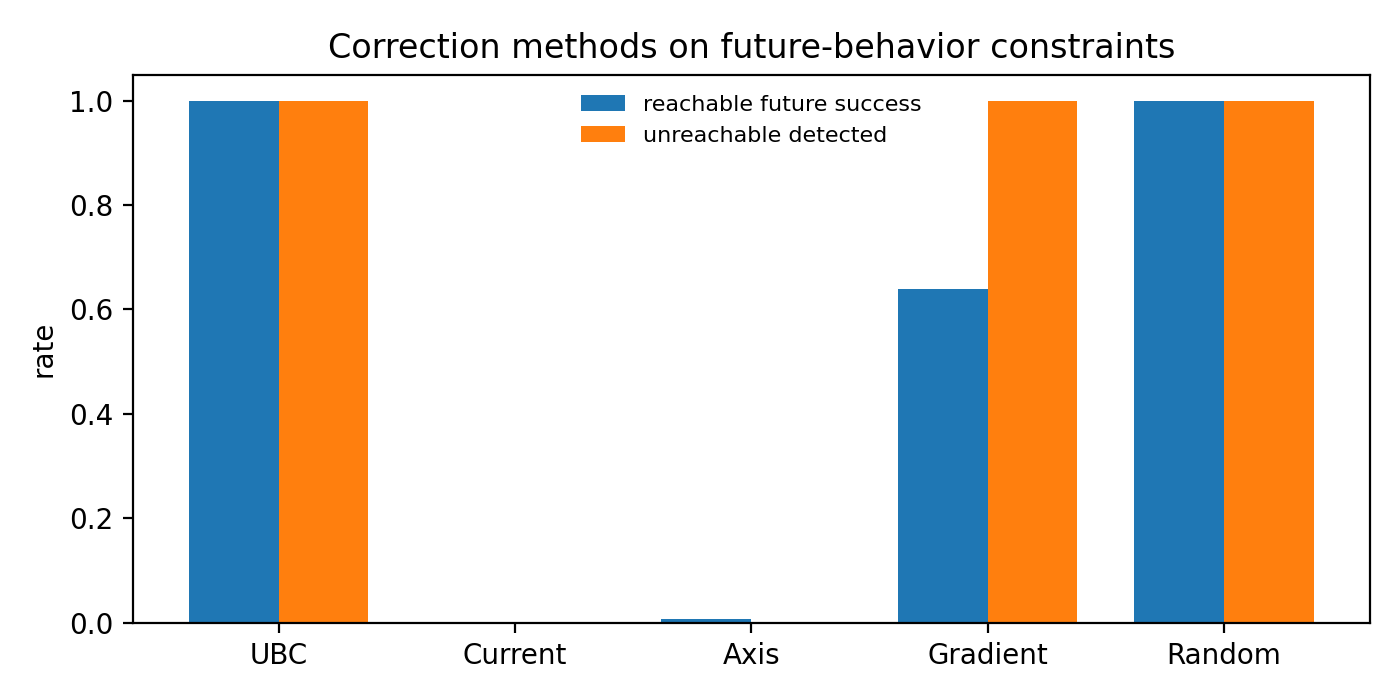
\includegraphics[width=\linewidth]{figures/success_rates.png}
\end{minipage}
\begin{minipage}{0.48\linewidth}
\centering
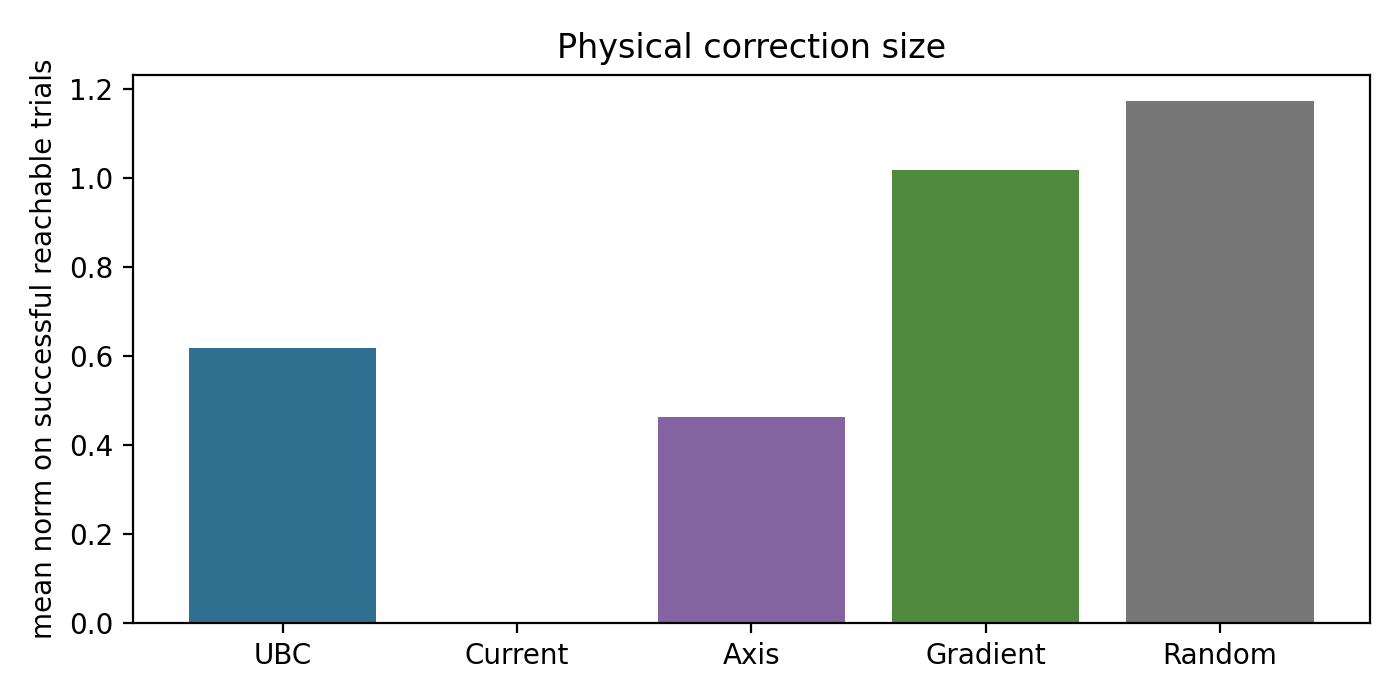
\includegraphics[width=\linewidth]{figures/correction_norms.png}
\end{minipage}
\caption{Left: future success and unreachable detection. Right: physical correction norm on successful reachable trials.}
\label{fig:results}
\end{figure}

The result is the intended stress test. Current-only corrections can satisfy the immediate margin while failing the future-context set. UBC succeeds on reachable local problems because it solves the exact projected halfspace problem; on contradictory problems it reports infeasibility. This is not evidence that UBC is a complete robot teacher. It is evidence that the distinction between current repair and future-behavior change is operational and measurable.

Table~\ref{tab:channel-noise} attacks the strongest hidden assumption: the robot must
know the local update channel. If UBC optimizes against $\hat H=H+\eta$ but the true
future margins are checked under $H$, the tight minimum-norm certificate becomes brittle.
At $\sigma=0.10$, unguarded success is 0.330. Adding a small uniform margin guard raises
success to 0.750, but it changes the object from minimum correction to a more conservative
correction. Thus UBC is exact for the modeled channel, not automatically robust to
Jacobian-estimation error.

\section{Limitations}
The guarantee is local to the affine update and linearized future-margin model. The finite context set $\mathcal{Z}$ is chosen by the designer and may miss deployment cases. The correction cost is Euclidean in the simulator rather than biomechanical. The experiments are abstract and do not include hardware contact, tactile sensing, or a high-dimensional policy. These limitations are central to the paper's honest scope: MEC is a formal object and UBC is a local certificate, not a universal account of human teaching.
The v2 estimated-channel stress adds a sharper boundary: if the update Jacobian is noisy,
the exact local certificate can fail on the true margins unless extra guard margins or
online validation are added.

\section{Conclusion}
Physical correction papers often conflate immediate repair with future robot learning. Minimum Effective Correction separates them. By projecting physical effort through the robot's update channel, UBC identifies the smallest correction that can change future behavior under a local model, and it exposes when the interface cannot provide such a correction. The mechanism is small, but the shift is sharp: the central question becomes not only what the human intended, but what the robot learner can actually absorb.

\bibliographystyle{iclr2026_conference}
\bibliography{references}

\appendix
\section{Proof Details}
\label{app:proof}
Consider $C=\{c:Hc\ge h\}$. If $C$ is nonempty, it is closed and convex. The function $f(c)=\frac12\|c\|_2^2$ is strongly convex, so it has at most one minimizer on $C$. Since $C$ is closed and $f$ is coercive, the minimizer exists. Therefore the solution of Equation~\ref{eq:ubc} is the unique minimum-norm correction in the local model.

If $C$ is empty, then by definition there is no correction vector satisfying all local future-margin constraints. This is a statement about the current correction channel $H=AJ$, not about the task in general. A different learner, feature map, or teaching interface can change $H$.

For the nullspace claim, let $v\in\mathrm{Null}(H)$. For any candidate correction $c$, the certified margin vector changes from $Hc-h$ to $H(c+v)-h=Hc-h$. Thus effort along $v$ may change contact geometry or compliance, but it cannot change the certified future margins under the modeled learner. This is the formal reason a visually meaningful physical correction can still be learning-irrelevant.

\section{Reproducibility}
The experiment can be rerun with:
\begin{verbatim}
python scripts/run_experiments.py
\end{verbatim}
The literature matrix and synthesis documents can be regenerated with:
\begin{verbatim}
python scripts/literature_pipeline.py
python scripts/synthesize_docs.py
\end{verbatim}

\end{document}
